% !TEX root = ../sommaire.tex

\chapter{Attribute Inference Attacks for Federated Regression Tasks}\label{chap:aia}

This chapter is based on our work \citeA{aia_regression}, published at the Thirty-Ninth AAAI Conference on Artificial Intelligence (AAAI 2025).

\paragraph{Chapter Summary}
Attribute inference attacks in federated learning have primarily been designed and evaluated for classification tasks~\cite{lyu2021novelattributereconstructionattack, chen2024practical}, leaving their effectiveness against regression models largely unexplored. In this chapter, we show that the limited performance of existing gradient-based attacks on regression tasks should not be interpreted as evidence of stronger privacy. Instead, we demonstrate that federated regression models are vulnerable to a different class of attacks based on the learned model itself. We introduce a two-stage model-based attribute inference attack in which the adversary first reconstructs or approximates the optimal local model of a targeted client and subsequently uses this model to infer sensitive attributes from the publicly known components of the client’s records. We develop attacks for both passive adversaries, who only observe the messages exchanged during training, and active adversaries, who can manipulate the models sent to the targeted client. For least-squares regression, we provide theoretical guarantees relating attack accuracy to the local model’s training error and derive conditions under which the client’s optimal local model can be reconstructed. Experiments on real-world datasets show that the proposed attacks consistently outperform existing gradient-based approaches, particularly under heterogeneous client data distributions and in settings where previous attacks approach random-guessing accuracy. These results establish model-based attacks as stronger and more appropriate baselines for empirically assessing privacy leakage in federated regression tasks.
\section{Motivation}

In Section~\ref{sec:privacy_in_fl}, we discussed how the repeated exchange of model updates in federated learning creates an additional attack surface during training. In particular, even when raw data remain local, the information exchanged during training may allow an adversary to infer sensitive attributes of a record from other attributes that are already known. This setting is especially relevant when records are only partially disclosed: for instance, in healthcare applications, some demographic or clinical information may be available while more sensitive attributes remain confidential. Recovering these withheld attributes can therefore constitute a meaningful privacy violation. Attribute inference attacks (AIAs) have been proposed precisely to study this type of leakage in federated learning~\cite{lyu2021novelattributereconstructionattack,chen2024practical}. Existing work, however, has focused primarily on classification tasks, leaving the privacy risks of \textit{regression} tasks largely unexplored, despite their widespread use in practical applications.

To investigate this gap, we compare in a preliminary experiment different AIAs on the ACS Income dataset~\cite{income_dataset}. Four clients train a neural network with a single hidden layer of 128 ReLU neurons through FedAvg, using one local epoch and a batch size of 32. Each client holds $S_u$ samples, and the adversary attempts to infer the gender attribute of every record from the remaining public information. We consider two learning tasks defined over the same data: a regression task that predicts an individual’s income, and a classification task that predicts whether the income exceeds the dataset median of $39\$K$, with label $\indicator_{y_i>39K}$ for sample $i$.
Quite surprisingly, the results in Figure~\ref{fig:gradient_vs_model}, demonstrate that the accuracy of state-of-the-art gradient-based AIA under a honest-but-curious adversary~\cite{lyu2021novelattributereconstructionattack, chen2024practical} (referred to as passive) drops significantly from $71\%$ on a classification task to $50\%$ (random guess) on a regression task once the targeted client holds more than 256 data points.
Furthermore,  even a more powerful (active) adversary capable of forging the messages to the targeted client to extract more information~\cite{lyu2021novelattributereconstructionattack, chen2024practical} offers only limited improvement to the AIA performance on regression tasks.


\begin{figure}[t]
    \centering
    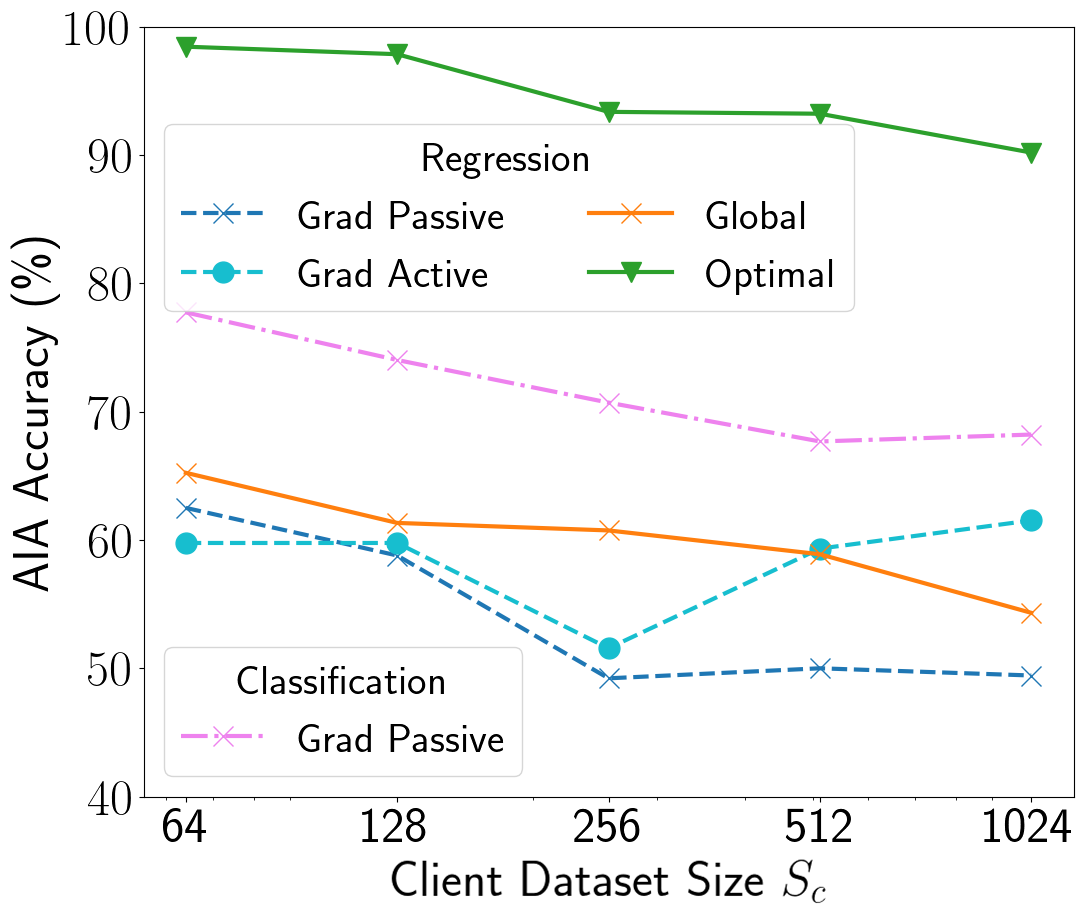
\includegraphics[scale=0.3]{assets/chapter_2/dataset_size_effect.png}
    \caption{Average performance of different AIAs when four clients train a neural network through FedAvg with 1 local epoch and batch size 32. Each client stores $S_u$ data points randomly sampled from the ACS Income dataset. The adversary infers the gender attribute of every data sample held by the client given access to the released (public) information.}
\label{fig:gradient_vs_model}
\end{figure}
In this chapter, we show that federated training of regression tasks does not inherently enjoy higher privacy, but it is simply more vulnerable to other forms of attacks. While existing FL AIA attacks for classification tasks are gradient-based, we show that model-based AIAs---initially proposed for centralized training~\cite{kasiviswanathan2013power, aia_fredrikson, yeom2018privacyriskmachinelearning, mehnaz2022sensitiveattributesprivatenovel}---may be more effective for regression tasks. Figure~\ref{fig:gradient_vs_model} illustrates that a model-based attack on the server's global model (i.e., the final model trained through FL) already performs at least as well as the SOTA gradient-based passive attack. Moreover, it highlights that even more powerful attacks (up to 30~p.p.~more accurate) could be launched if the adversary had access to the optimal local model of the targeted client (i.e., a model trained only on the client's dataset).

Motivated by these observations, we propose a new two-step model-based AIA for \emph{federated regression tasks}. In this attack, the adversary first (approximately) reconstructs the client's optimal local model and then applies an existing model-based AIA to that model.

Our main contributions can be summarized as follows:
\begin{itemize}
    \item  We provide an analytical lower bound for model-based AIA accuracy in the least squares regression problem. This result motivates the adversary's strategy to approximate the client's optimal local model in federated regression tasks (Sec.~\ref{sec:model-based-guarantees}).
    \item   We propose methods for approximating optimal local models where adversaries can either eavesdrop on exchanged messages or directly interfere with the training process (Sec.~\ref{sec:lmra}).  
    \item Our experiments show that our model-based AIAs are better candidates for empirically quantifying privacy leakage for federated regression tasks  (Sec.~\ref{sec:exp}).
\end{itemize}

\section{Problem Description and Background}
\subsection{Federated Learning}

We consider here the same problem formulation described in Section~\ref{sec:fed_learning}. We denote by $\clients$ the set of all clients participating to FL. 
Let $\localdataset = \{(\x_u(i), y_u(i)), i=1,\dots, S_u\}$ denote the local dataset of client $u\in \clients$ with size $S_u\triangleq |\localdataset|$.  Each data sample $(\x_u(i), y_u(i))$ is a pair consisting of an input $\x_u(i)$ and of an associated target value $y_u(i)$.
In FL, clients cooperate to learn a global model, which minimizes the following empirical risk over all the data owned by clients:
\begin{equation}
\label{eq:globalobjective}
\min_{\model \in \real^d} \globallossfunction(\model) 
= \sum_{u \in \clients} p_u \locallossfunction(\model, \dataset_u)
= \sum_{u \in \clients} p_u \left( \frac{1}{S_u} \sum_{i=1}^{S_u} \ell(\model, \x_u(i), y_u(i)) \right),
\end{equation}
where $\ell(\model, \x_u(i), y_u(i))$ measures the loss of the model $\model$ on the sample $(\x_u(i), y_u(i))\in \localdataset$ and $p_u$ is the positive weight of client $u$, s.t.,~$\sum_{u\in \clients} p_u = 1$. Common choices of weights are $p_u =\frac{1}{|\clients|}$ or $p_u =\frac{S_u}{\sum_{u\in \clients}S_u}$.


Let $\model^\star = \arg\min_{\model \in \real^d} \globallossfunction(\model)$ be a global optimal model, i.e., a minimizer of Problem~\eqref{eq:globalobjective}. 
A general framework to learn such a global model in a federated way is shown in Algorithm~\ref{algo:fl-framework}; it generalizes a large number of FL algorithms, including FedAvg~\cite{pmlr-v54-mcmahan17a}, FedProx~\cite{fedprox}, and FL with different client sampling techniques~\cite{nishio2019client, chen2020optimal, cho2020client}. The model~$\model^T$---the output of Algorithm~\ref{algo:fl-framework}---is the tentative solution of Problem~\eqref{eq:globalobjective}. Its performance depends on the specific FL algorithm, which specifies how clients are selected in line~\ref{algoline:select_client}, how the updated local models are aggregated in line~\ref{algoline:aggregation}, and how the local update rule works in line~\ref{algoline:updaterule}.

\subsection{Threat Model}\label{subsection:threadmodel}

\subsubsection{Honest-but-Curious Adversary}
We describe first an honest-but-curious adversary,\footnote{In what follows, we refer to the client using female pronouns and the adversary using male pronouns, respectively.} which is a standard threat model in existing literature~\cite{melis2018exploitingunintendedfeatureleakage,geiping_ig, yinSeeGradientsImage2021,Nasr2018ComprehensivePA}, including the FL one~\cite[Table~7]{kairouz_open_problems}, 
\cite{lyu2021novelattributereconstructionattack, chen2024practical}. This \emph{passive} adversary, who could be the server itself, is 
knowledgeable about the trained model structure, the loss function, and the training algorithm, and may eavesdrop on communication between the attacked client and the server but does not interfere with the training process. For instance, during training round $t$, the adversary can inspect the messages exchanged between the server and the attacked client (denoted by $u$), allowing him to recover the parameters of the global model $\model^t$ and the updated client model $\model_u^t(K)$. %NOTE: I removed the citation to the algorithm that we have in the Appendix. 
Let $\roundsclient \subseteq \{t|u\in\clients^t, \forall t\in {0,\dots,T-1}\}$ denote the set of communication rounds during which the adversary inspects messages exchanged between the server and the attacked client and $\messages_u = \{(\model^t, \model_u^t), \forall t\in \roundsclient\}$ denote the corresponding set of messages.

When it comes to defenses against such an adversary, it is crucial to understand that traditional measures like encrypted communications are ineffective if the attacker is the FL server.
More sophisticated cryptographic techniques like secure aggregation protocols~\cite{secure_aggregation_bonawitz, kadhe2020fastsecagg} allow the server to aggregate local updates without having access to each individual update and, then, do hide the client's updated model $\model_u^t$ from the server. Nevertheless, they come with a significant computation overhead~\cite{quoc2020securetf} and are inefficient for sparse vector aggregation~\cite{kairouz_open_problems}. Moreover, they are vulnerable to poisoning attacks, as they hinder the server from detecting (and removing) potentially harmful updates from malicious clients~\cite{blanchard_byz, yin2018byzantine,mhamdi2018hiddenvulnerabilitydistributedlearning}. For instance, \citeA[Sec.~4.4]{truthSerum} introduce a new class of data poisoning attacks that succeed when training models with secure multiparty computation. Alternatively, Trusted Execution Environments (TEEs) ~\cite{TEE, tee2} provide an encrypted memory region to ensure the code has been executed faithfully and privately. They can then both conceal clients' updated models and defend against poisoning attacks. However, implementing a reliable TEE platform in FL remains an open challenge due to the infrastructure resource constraints and the required communication processes needed to connect verified codes~\cite{kairouz_open_problems}.


\subsubsection{Malicious Adversary} 
We also consider a stronger \emph{active} adversary who can interfere with the training process. Specifically, this adversary can modify the messages sent to the clients and have the clients update models~$\model^t$ that have been concocted to reveal more private information. 
 Let $\mathcal{T}^a_u $ be the set of rounds during which the adversary attacks client $u$ by sending a malicious model $\model^t$. 
As above, the adversary could be the server itself. As discussed in Section~\ref{sec:privacy_in_fl}, this adversary has been widely considered in the literature on reconstruction attacks~\cite{wenFishingUserData2022a,boenischWhenCuriousAbandon2023} and membership inference attacks~\cite{mia_nguyen, Nasr2018ComprehensivePA}. Some studies have also explored the possibility of a malicious adversary modifying the model architecture during training~\cite{fowlRobbingFedDirectly2021,zhaoLOKILargescaleData2023a}, even though such attacks appear to be easily detectable. Here, we do not allow the adversary to modify the model architecture. 
For simplicity, we will refer to these two adversaries as passive and active adversaries, respectively, throughout the rest of the chapter.

\subsection{Attribute Inference Attack (AIA) for FL}

As presented in Section~\ref{sec:aia}, an AIA leverages public information to infer private or sensitive attributes~\cite{kasiviswanathan2013power,aia_fredrikson, yeom2018privacyriskmachinelearning,lyu2021novelattributereconstructionattack,chen2024practical}.
Formally, each input $\x_u(i)$ of client $u$ consists of public attributes $\x_u^p(i)$ and a sensitive attribute $s_u(i)$. The target value, assumed to be public, is denoted by $y_u^p(i)$. The adversary has access to
\[
    \{(\x_u^p(i),y_u^p(i))\}_{i=1}^{S_u}
\]
and to the exchanged messages $\messages_u$, and aims to recover the sensitive attributes $\{s_u(i)\}_{i=1}^{S_u}$. Unlike the stronger adversaries considered in~\cite{aia_fredrikson,yeom2018privacyriskmachinelearning}, we do not assume access to estimates of the marginal or joint distribution of the data.

% As presented in Section~\ref{sec:aia}, AIA leverages public information to deduce private or sensitive attributes~\cite{kasiviswanathan2013power,fraia_fredrikson, yeyeom2018privacyriskmachinelearning,lyu2021novelattributereconstructionattack, chen2024practical}.
% % For example, an AIA could reconstruct a user's gender from a recommender model by having access to the user's provided ratings.
% Formally, each input $\x_u(i)$ of client $u$ consists of public attributes $\x_u^p(i)$ and of a sensitive attribute~$s_u(i)$. The target value, assumed to be public, is denoted by $y_u^p(i)$. The adversary, having access to $\{(\x_u^p(i), y_u^p(i)), i=1,..., S_u\}$ and $\messages_u$, aims to recover the sensitive attributes ${s_u(i)}$.\footnote{In ~\cite{fredrikson2014privacy, yeom2018privacy}, the adversary possesses additional information, including
% estimates of the marginals or the joint distribution of the data samples. However, in this chapter, we do not consider such a more powerful adversary.}
%~\cite{kasiviswanathan2013power, attribute_fl}.

\subsubsection{Existing Gradient-Based AIA for FL.}\label{subsec:gradient-based}
 \citeA{lyu2021novelattributereconstructionattack} and \citeA{chen2024practical} present AIAs specifically designed for the FL context and both passive and active adversaries.
The central idea involves identifying sensitive attribute values that yield virtual gradients closely resembling the client's model updates---referred to as \emph{pseudo-gradients}---in terms of cosine similarity. F Formally, the adversary solves the following optimization problem:
 \begin{equation}\label{eq:aia_gradient_based}
  \argmax_{\{s_u(i)\}_{i=1}^{S_u}} \sum_{t\in \mathcal{T}}\textbf{CosSim} \left(\frac{\partial\ell(\model^t, 
    \{(\x_u^p(i), s_u(i), y_u^p(i))\})}{\partial \model^t}, \model^t-\model_u^t\right), 
\end{equation}
where $\mathcal{T}\subseteq \mathcal{T}_u$ for a passive adversary and  $\mathcal{T}\subseteq \mathcal{T}_u \cup \mathcal{T}_u^a$ for an active adversary. 
The active adversary simply sends back to the targeted client $u$ her own model $\model_u^{(t-1)}$ at each attack round in $\mathcal{T}_u^a$.

\citeA{lyu2021novelattributereconstructionattack} and \citeA{chen2024practical} assume that the sensitive attributes are categorical. 
%and discrete random variables. 
Nevertheless, problem~\eqref{eq:aia_gradient_based} can be solved efficiently using a gradient method with the reparameterization trick and the Gumbel softmax distribution~\cite{jang2017categorical}. 
From~\eqref{eq:aia_gradient_based}, we observe that, since gradients incorporate information from all samples, the attack performance deteriorates in the presence of a large local dataset.
For example, the attack accuracy almost halves on the Genome dataset for the classification task when the client's local dataset size increases from 50 to 1000 samples~\cite[Table~8]{lyu2021novelattributereconstructionattack}. Our experiment (Figure~\ref{fig:gradient_vs_model}) on a regression task corroborates this finding: when the local dataset size increases from 64 to 256, the attack accuracy drops from $60\%$ to the level of random guessing.

\subsubsection{Model-Based AIA} As an alternative, the AIA can be executed directly on the model (rather than on the model pseudo-gradients), as initially proposed for  centralized training in~\cite{kasiviswanathan2013power,aia_fredrikson}. Given a model $\model$, the adversary can infer the sensitive attributes by solving the optimization problems presented in Equation~\ref{eq:aia_mb}, here reformulated to align the notation:
\begin{equation}\label{eq:aia_model_based}
     \argmin_{s_u(i)} \ell(\model,(\x_u^p(i), s_u(i), y_u^p(i))),\,\,\, \forall i\in\{1,\dots,S_u\}, 
\end{equation}

Below we provide theoretical guarantees (Prop.~\ref{prop:attribute_nonprivate}) for the accuracy of model-based AIAs to least squares regression problems. %Our theoretical result supports , in an FL setting, the adversary may advantageously start by estimating the client's optimal local model, i.e., the model that minimizes the client's empirical loss.
Our theoretical result corroborates that, in an FL setting,  an adversary can benefit by first estimating the client’s optimal local model---that is, the model that minimizes the client’s empirical loss.

\section{Model-Based AIA Guarantees for Least Squares Regression}
\label{sec:model-based-guarantees}
In this section, we provide novel theoretical guarantees for the accuracy of the model-based AIA (Problem~\eqref{eq:aia_model_based}) in the context of least squares regression. In particular, we show that the better the model $\model$ fits the local data and the more the sensitive attribute affects the final prediction, the higher the AIA accuracy.
 \begin{prop}\label{prop:attribute_nonprivate}
Let $E_u$ be the mean square error of a given least squares regression model $\model$ on the local dataset of client $u$ and $\model[s]$ be the model parameter corresponding to a binary sensitive attribute. The accuracy of the model-based AIA \eqref{eq:aia_model_based} is larger than or equal to $1-\frac{4E_u}{\model[s]^2}$. 
\end{prop}

\begin{proof}
Let $\s $ be the vector including all the unknown sensitive binary attributes $\{s_u(i), \forall i\in \{1, ..., S_u\}\}$ of client $u$.
Let $\x_u\in \real^{S_u\times d}$ be the design matrix with rank $d$ and $\y\in \real^{S_u}$ be the labels in the local dataset $\localdataset$ of the client $u$.  Let $\model[:p]\in \real^{d-1}$ be the parameters corresponding to the public attributes. 
The adversary has access to partial data instances in $\localdataset$ which consists of the public attributes $\P\in \real^{S_u\times(d-1)}$ and the corresponding labels $\y\in \real^{S_u}$. 

The goal for the adversary is to decode the values of the binary sensitive attribute $\s \in\{0,1\}^{S_u}$ given $(\P, \y)$ by solving~\eqref{eq:aia_model_based}, i.e., checking for each point, which value for the sensitive attribute leads to a smaller loss.

It is easy to verify that the problem can be equivalently solved through the following two-step procedure.
First, the adversary computes the vector of real values:
$$
\tilde{\mathbf{s}}_u = \argmin_{\s\in \real^{S_u}} ||\P\model[:p]+ \s\model[s] - \y ||_2^2 = \frac{\y-\P\model[:p]}{\model[s]}.  
$$
Then, the adversary reconstruct the vector of sensitive features $\hat{\mathbf{s}}_u \in \{0,1\}^{S_u}$ as follows
\begin{equation}\label{eq:sensitive_prediction_condition}
\hat s_u(i) = 
\begin{cases}
    0& \text{if } \tilde{{s}}_u(i) <\frac{1}{2}\\
    1              & \text{otherwise}
\end{cases}
,\,\,\,\forall i\in \{1, ..., S_u\}. 
\end{equation}

Let $\e$ be the vector of residuals for the local dataset, i.e., $\e_u = \y - (\P\model[:p]+ \s\model[s])$. We have then 
\begin{equation}\label{eq:sensitive_relation}
    \s = \frac{\y - \P \model[:p] - \e_u}{\model[s]} = \tilde{\mathbf{s}}_u - \frac{\e_u}{\model[s]}. 
\end{equation}

Let us say that the sensitive feature of sample $i$ has been erroneously reconstructed, i.e., $s_u(i) \neq \hat s_u(i)$, then  \eqref{eq:sensitive_prediction_condition}, implies that $|s_u(i) - \tilde s_u(i)|\ge 1/2$, and from
 \eqref{eq:sensitive_relation} it follows that $|e_u(i)|^2 \ge \model[s]^2/4$. As $E_u S_u= \lVert \e_u \rVert_2^2$, there can be at most $4 E_u S_u/\model[s]^2$ samples erroneously reconstructed, from which we can conclude the result.
 \end{proof}

Proposition~\ref{prop:attribute_nonprivate} indicates that the model-based AIA performs better the more the model overfits the dataset.
This observation justifies the following two-step attack in a FL setting: 
\emph{the adversary first reconstructs the optimal local model of the targeted client $u$, i.e., $\localmodel = \arg\min_{\model\in \real^d} \locallossfunction(\model, \localdataset)$, and then execute the AIA in \eqref{eq:aia_model_based} on the reconstructed model.} Here, the term \emph{optimal local model} refers to the model that minimizes the empirical loss on the client’s local dataset; it does not imply optimal test performance and, on the contrary, likely corresponds to an overfitted model.

% \footnote{
% Note that this model is optimal in terms of the training error, but not in general of the final test error. On the contrary, it is likely to overfit the local dataset.

In the following, we will detail our approaches for reconstructing the optimal local model by passive and active adversary, respectively.   

\section{Reconstructing the Local Model in FL}\label{sec:lmra}
In this section, we show how an adversary may reconstruct the optimal local model of client $u$, i.e.,~$\localmodel = \arg\min_{\model\in \real^d} \locallossfunction(\model, \localdataset)$.

First, we provide an efficient approach for least squares regression under a passive adversary. We prove that the adversary can exactly reconstruct the optimal local model under deterministic FL updates and provide probabilistic guarantees on the reconstruction error under stochastic FL updates (Sec.~\ref{sec:exact}).

Second, we show that an active adversary can potentially reconstruct any client's local model (not just least square regression ones) in a federated setting (Sec.~\ref{subsec:active}).


\subsection{Passive Approach for Linear Least Squares}\label{sec:exact}

We consider that clients cooperatively train a linear regression model with quadratic loss. We refer to this setting as a federated least squares regression.  % $\localdataset$.
The attack is detailed in Algorithm~\ref{algo:lineardecode} and  involves a single matrix computation (line~\ref{algoline:ols}) after the exchanged messages $\messages_u$ have been collected. $\mathbf{A}^\dagger$ represents the pseudo-inverse of matrix $\mathbf{A}$.  
Theorem~\ref{prop:stochastic_case} provides theoretical guarantees for the distance between the reconstructed model and the optimal local one, when the model is trained through FedAvg~\cite{pmlr-v54-mcmahan17a} with batch size $B$ and local epochs $E$. The proof can be found in Appendix~\ref{app:stochasticproof}

\begin{savenotes}
\begin{theorem}\label{prop:stochastic_case}
Consider training a least squares regression through FedAvg (Algorithm~\ref{algo:fedavg}) with batch size $B$ and local epochs $E$. Assume that 
\begin{enumerate}
    \item the client's design matrix $\x_u\in \real^{S_u\times d}$ has rank $d$ equal to the number of features plus one;\footnote{Remember that a client's design matrix has a number of rows equal to the input features of the samples in the client's local training dataset.}
    \item the components of the stochastic (mini-batch) gradient are distributed as sub-Gaussian random variables with variance proxy $\sigma^2$, i.e.,
    \[
        \E\!\left[\exp\!\left(\frac{\ei[i]}{\sigma^2}\right)\right]
        \leq \exp(1),
        \qquad \forall \model,\quad \forall i\in\{1,\dots,d\},
    \]
    where $\ei = \gradient(\model) - \nabla \locallossfunction(\model)$;\footnote{This condition implies a bounded variance for each component of the stochastic gradient.}
\item the input model vectors at an observed round are independent of the previous stochastic gradients computed by the attacked client;
\item there exists $\underline{\lambda}>0$ such that $\forall n_u \in \mathbb{N}$, we can always select $n_u$ observation rounds so that $\lambda_{\min}\!\left(\frac{\Theta_{\text{out}}^{T} \Theta_{\text{out}}}{n_u}\right) \ge \underline{\lambda}$, where $\lambda_{\min}(\mathbf{A})$ denotes the smallest eigenvalue of the matrix $\mathbf{A}$, and $\Theta_{\text{out}}$ is defined in Algorithm~\ref{algo:lineardecode}.
\end{enumerate}
%the variance of the stochastic (mini-batch) gradient is bounded,~s.t.
%\[
%\E [\left\lVert \gradient(\model) - \nabla \locallossfunction(\model) \right\rVert^2_2 \leq \sigma^2], \forall \model,
%\]
The error of the reconstructed model $\hat\model^*_u$ of Algorithm~\ref{algo:lineardecode} is upper bounded w.p.  $\ge 1-\delta$  when $\eta\leq \frac{S_u}{2\lambda_{\max}(\x_u^T\x_u)}$ and
\begin{equation}
   \left\lVert \hat\model^*_u - \localmodel \right\rVert_2 = \mathcal{O}\left(\eta\sigma d\sqrt{ d E\left\lceil\frac{S_u}{B}\right\rceil \frac{d+1+\ln \frac{2d}{\delta}}{n_u \cdot \underline{\lambda}}} \right). 
\end{equation}
\end{theorem}
\end{savenotes}


When the batch size is equal to the local dataset size, Algorithm~\ref{algo:lineardecode} exactly reconstructs the optimal local model (proof in Appendix\ref{app:proof_corollary}):

\begin{prop}\label{cor:linear_reconstruction}
Consider a federated least squares regression and assume that client $u$ has $d$-rank design matrix and updates the global model through full-batch gradient updates (i.e., $B=S_u$) and an arbitrary number of local epochs. Once the adversary eavesdrops on $d+1$ communication exchanges between client $u$ and the server, he can recover the client's optimal local model.
\end{prop}

Finally, the following proposition shows that 
our attack for the full-batch gradient case is \textbf{order-optimal} in terms of the number of messages the adversary needs to eavesdrop. The proof is in Appendix~\ref{app:proof_proposition}.

\begin{prop}\label{prop:order-optimal}
Consider that the federated least squares regression is trained through FedAvg with one local step ($E=1$) and full batch ($B=S_u$ for each client $u \in \mathcal{U}$). At least one client is required to communicate with the server $\Omega(d)$ times for the global model to be learned, and the adversary needs to eavesdrop at least $\Omega(d)$ messages from this client to reconstruct her optimal local model.
\end{prop}

\begin{algorithm2e}[H]
\caption{Reconstruction of client-$u$ local model by a passive adversary for federated least-squares regression}
\label{algo:lineardecode}
\KwInput{server models $\model^{t_i}(0)=\model_u^{t_i}(0)$ and local updated models $\model_u^{t_i}(K)$ at the inspected rounds $t_i \in \mathcal{T}_u = \{t_1,t_2,\dots,t_{n_u}\}$}

$\Theta_{\text{in}} \leftarrow [\model_u^{t_1}(0)\; \model_u^{t_2}(0)\; \dots\; \model_u^{t_{n_u}}(0)]^T \in \real^{n_u \times d}$\;

$\Theta_{\text{out}} \leftarrow
\left[
\begin{array}{cc}
(\model_u^{t_1}(0)-\model_u^{t_1}(K))^T & 1 \\
\vdots & \vdots \\
(\model_u^{t_{n_u}}(0)-\model_u^{t_{n_u}}(K))^T & 1
\end{array}
\right] \in \real^{n_u \times (d+1)}$\;

$(\hat\model_u^*)^T \leftarrow \text{last row of }\left((\Theta_{\text{out}}^T \Theta_{\text{out}})^\dagger \Theta_{\text{out}}^T \Theta_{\text{in}}\right)$\;
\label{algoline:ols}

\Return{$\hat\model_u^*$ as the estimator for client $u$'s local model}\;
\end{algorithm2e}

\paragraph{Toy Example Illustration.} 
Here, we illustrate the performance of our Algorithm~\ref{algo:lineardecode} on a toy dataset detailed in Appendix~\ref{app:toydataset}. Figure~\ref{fig:linear_toy} (left) demonstrates that 
as the batch size increases, the reconstructed model is closer to the optimal local model (as shown in our Theorem~\ref{prop:stochastic_case}). Moreover, since the model overfits more the dataset (with smaller loss), the AIA accuracy increases (Figure~\ref{fig:linear_toy} (right)). 
\begin{figure}[htbp]
\begin{subfigure}[t]{0.45\columnwidth}
    \centering
    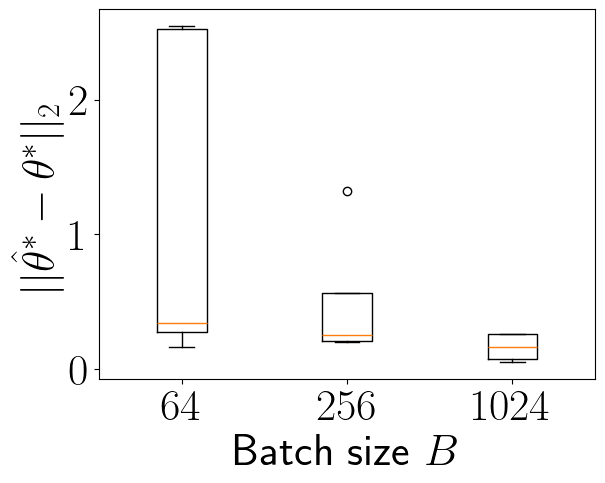
\includegraphics[scale=0.4]{assets/chapter_2/Passive_linear_LMRA_1.png}
\end{subfigure}
\begin{subfigure}[t]{0.45\columnwidth}
    \centering
    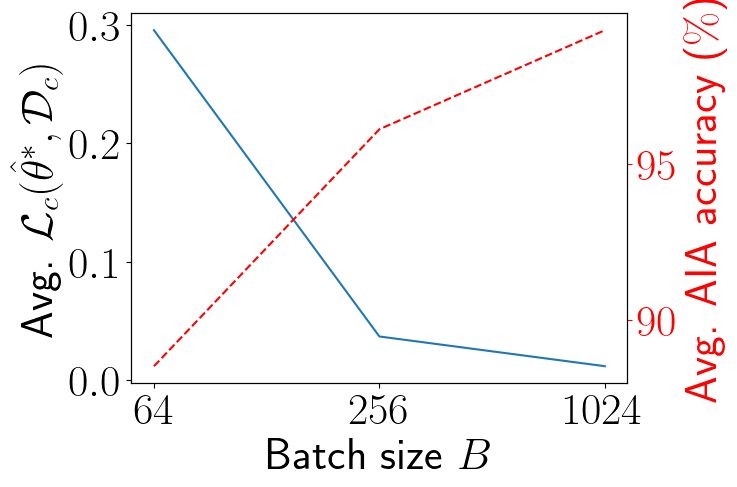
\includegraphics[scale=0.4]{assets/chapter_2/Passive_linear_AIA_1.png}
\end{subfigure}
\caption{The performance of our passive approach for reconstructing optimal local model (left) and the triggered AIA (right) on a toy dataset with two clients training a linear model with size $d=11$ under batch size 64, 256 and 1024 for 5 seeds each, respectively. The passive adversary only eavesdropped $d+1$ messages.}
\label{fig:linear_toy}
\end{figure}


\subsection{Active Approach} \label{subsec:active}
Here we consider an active adversary (e.g., the server itself) that can modify the global model weights $\model^t$ to recover the client's optimal local model. 
To achieve this, the adversary can simply send back to the targeted client $u$ her own model $\model_u^{(t-1)}$ instead of the averaged model $\model^t$. In this way, client $u$ is led to compute her own optimal local model.

We propose a slightly more sophisticated version of this active attack. Specifically, we suggest that the adversary emulates the Adam optimization algorithm~\cite{adam} for the model updated by client $u$ by adjusting the learning rate for each parameter based on the magnitude and history of the gradients, and incorporating momentum. The motivation is twofold. First, the client does not receive back exactly the same model and thus cannot easily detect the attack. Second, Adam is known to minimize the training error faster than stochastic gradient descent at the cost of overfitting more to the training data~\cite{adam_generalize_1, adam_generalize}. We can then expect Adam to help the adversary reconstruct the client's optimal local model better for a given number of modified messages, and our experiments in Sec.~\ref{sec:exp}
 confirm that this is the case.

The details of this attack are outlined in Algorithm~\ref{algo:active}. We observe that the adversary does not need to systematically modify all messages sent to the target client $u$ but can modify just a handful of messages that are not necessarily consecutive. This contributes to the difficulty of detecting the attack.

\begin{algorithm2e}[H]
  \caption{Reconstruction of client-$u$'s local model by an active adversary $a$}
  \label{algo:active}

  \KwInput{attack rounds $\mathcal{T}_u^a$ for client $u$; corresponding malicious model $\model_u^a$}

  $\model_u^a \leftarrow$ latest model received from client $u$\;

  \For{$t \in \mathcal{T}_u^a$}{
      $a$ sends the model $\model_u^a$ to client $u$\;

      $a$ waits for the updated model $\model_u$ from client $u$\;

      $a$ computes the pseudo-gradient $\model_u^a - \model_u$ and updates
      $\model_u^a$ and the corresponding moment vectors following Adam~\cite[Algorithm~1]{adam}\;
  }

  \Return{$\model_u^a$ as the estimator for client $u$'s local model}\;
\end{algorithm2e}

\section{Experimental Evaluation}\label{sec:exp}
\subsection{Datasets} \label{subsec:datasets}
\paragraph{Medical}~\cite{medical_dataset}. This dataset includes 1,339 records and 6 features: age, gender, BMI, number of children, smoking status, and region. The \emph{regression} task is to predict each individual's medical charges billed by health insurance. The dataset is split i.i.d. between 2 clients.

\paragraph{Income}~\cite{income_dataset}. This dataset contains census information from 50 U.S. states and Puerto Rico, spanning from 2014 to 2018. It includes 15 features related to demographic information such as age, occupation, and education level.
The \emph{regression} task is to predict an individual's income. 
We investigate two FL scenarios, named \mbox{Income-L} and Income-A, respectively. In Income-L, there are 10 clients holding only records from the  state of Louisiana (15,982 records in total). These clients can be viewed as the local entities working for the Louisiana State Census Data Center. We examine various levels of statistical heterogeneity among these local entities, with the splitting strategy detailed in Appendix~\ref{app:datasplit_incomel}. In Income-A, there are 51 clients, each representing a census region and collectively covering all regions. Every client randomly selects 20\% of the data points from the corresponding census region, resulting in a total of 332,900 records.

For all the datasets, each client keeps $90\%$ of its data for training and uses $10\%$ for validation.

\subsection{Experimental Settings}
Across all experiments, the adversary infers the smoking status in the Medical dataset and gender in the Income-L and Income-A datasets. We measure attack performance using the AIA accuracy, defined as the fraction of sensitive attributes correctly inferred across all samples.

\subsubsection{Federated Least Squares Regression}
In these experiments, each client trains a linear least-squares regression model through FedAvg. For Income-L and Income-A, we simplify the feature representation to make the prediction task suitable for linear least-squares regression, mainly by removing high-cardinality categorical features and aggregating some categorical values. The complete preprocessing procedure is detailed in Appendix~\ref{app:hyperparameters}.

Training is performed for $T=300$ communication rounds, using one local epoch and a batch size of 32. Each client participates in all rounds, i.e., $\mathcal{T}_c=\{0,\ldots,T-1\}$, and the learning rate is fixed to $5\cdot10^{-3}$. The passive adversary may eavesdrop on all exchanged messages until the end of training, whereas the active adversary launches the attack after round $T$ for an additional 10 or 50 rounds. All attacks target a single client selected at random. To approximate the optimal local model of the targeted client, the passive adversary applies Algorithm~\ref{algo:lineardecode}, while the active adversary applies Algorithm~\ref{algo:active}. Every attack is evaluated over three FL training runs with different random seeds.

\subsubsection{Nerual Networks}
In all the experiments, each client follows FedAvg to train a neural network model with a single hidden layer of 128 neurons, using ReLU as activation function. 
The number of communication rounds is fixed to $T = \lceil 100/E \rceil$ where $E$ is the number of local epochs. Each client participates to all rounds, i.e.,~$\mathcal{T}_c = \{0,...,T-1\}$.
The learning rate is tuned for each training scenario (different datasets and number of local epochs), with values provided in Appendix~\ref{app:hyperparameters}. The passive adversary may eavesdrop all the exchanged messages until the end of the training. 
The active adversary launches the attack after $T$ rounds for additional $\lceil 10/E \rceil$ and $\lceil 50/E \rceil$ rounds.
Every attack is evaluated over FL trainings from 3 different random seeds.We also examine the impact of the attack's starting round. The results are presented in Appendix~\ref{app:starting_points}.


\subsection{Attack Methods and Baselines}\label{subsec:baseline}
\subsubsection{Gradient-Based}
We compare our method with the (gradient-based) SOTA (Sec.~\ref{subsec:gradient-based}). 
The baseline performance is affected by the set of  inspected rounds~$\mathcal{T}$ considered in~\eqref{eq:aia_gradient_based}. We select the inspected rounds $\mathcal{T}$ based on two criteria: the highest cosine similarity and the best AIA accuracy. In a real attack, the adversary is not expected to know the attack accuracy beforehand.
%for tuning purposes. 
Therefore,  we refer to the attack based on the highest cosine similarity as {\bf{Grad}}  and to the other as {\bf{Grad-w-O}} ({\bf Grad}ient {\bf w}ith {\bf O}racle), as it assumes the existence of an oracle that provides the attack accuracy. The details for the tuning of $\mathcal{T}$ and other hyper-parameter settings can be found in Appendix~\ref{app:hyperparameters}.
   
\subsubsection{Our Attacks} 
Our attacks consist of two steps: 1) approximating the optimal local model of the targeted client, and 2) executing the model-based AIA in~\eqref{eq:aia_model_based} on the reconstructed model. The first step depends on the considered model. For federated least squares regression, the passive adversary reconstructs the local model using Algorithm~\ref{algo:lineardecode}, whereas for neural networks it uses the last model returned by the targeted client. In both settings, the active adversary applies Algorithm~\ref{algo:active}. Further implementation details and hyperparameter configurations are provided in Appendix~\ref{app:hyperparameters}.

\paragraph{Model-Based with Oracle (Model-w-O).} 
To provide an upper bound on the performance of our approach, we assume the existence of an oracle that provides the optimal local model for the first step of our attack. In practice, the optimal local model is determined empirically by running Adam for a very large number of iterations.

\subsection{Experimental Results on Federated Least Squares Regression}

% Results in Table~\ref{tab:attack_linear} show that our attacks outperform the baseline Grad in both passive and active scenarios on across all three datasets. Notably, our passive attack achieves improvements of over 4, 5 and 7 percentage points (p.p.) for Income-L, Income-A and Medical datasets, respectively. Even when the gradient-based method has access to an oracle, our passive attacks still achieves higher accuracy on Income-A and Income-L and comes very close on Medical dataset. 
% More importantly, our passive attack reaches already  to the performance expected from an adversary who knows the optimal local model,  demonstrating the effectiveness of our passive approach in approximating the optimal local model (Algorithm~\ref{algo:lineardecode}).
% When shifting to active attacks,  the performance gain over Grad remains largely consistent after 50 active rounds.

Table~\ref{tab:attack_linear} reports the AIA accuracy for federated least-squares regression. We first consider the passive setting. Our attack consistently outperforms the realistic gradient-based baseline \textbf{Grad}, improving the AIA accuracy by approximately $6$, $7$, and $6$ percentage points (p.p.) on Income-L, Income-A, and Medical, respectively. Our approach also remains competitive with \textbf{Grad-w-O}, despite the latter relying on an oracle to select the attack rounds. In particular, our attack slightly outperforms Grad-w-O on Income-L and Income-A, while achieving a comparable accuracy on Medical.

More importantly, these experiments validate the local-model reconstruction strategy underlying our approach. The passive attack achieves $59.05\%$, $56.56\%$, and $94.13\%$ accuracy on Income-L, Income-A, and Medical, respectively, compared with $59.10\%$, $56.56\%$, and $94.13\%$ for Model-w-O. Hence, across all three datasets, the model reconstructed from the observed FL messages through Algorithm~\ref{algo:lineardecode} is sufficient to attain essentially the same AIA accuracy as direct access to the optimal local model. This provides empirical support for the theoretical analysis of the passive reconstruction approach and shows that, in the least-squares setting, the information contained in the exchanged models can be sufficient to recover most of the privacy leakage exposed by the client's local optimum.

The results also explain why granting additional capabilities to our adversary provides only limited benefits in this setting. Since the passive reconstruction already achieves near-oracle AIA performance, there is little room for the active procedure to further improve the attack. After 50 active rounds, our attack reaches $59.10\%$, $56.22\%$, and $93.91\%$ on the three datasets, remaining close to Model-w-O and approximately $6$ p.p. above the realistic Grad baseline.

\begin{table}[t]
    \centering
    \setlength{\tabcolsep}{6pt}
    \renewcommand{\arraystretch}{1.08}
    \begin{tabular}{@{}lccc@{}}
        \toprule
        \textbf{Attack} & \multicolumn{3}{c}{\textbf{Dataset}} \\
        \cmidrule(l){2-4}
        & \textbf{Income-L} & \textbf{Income-A} & \textbf{Medical} \\
        \midrule
        \multicolumn{4}{@{}l}{\textbf{Passive}} \\
        \quad Grad     & $53.10 \pm 1.40$          & $49.74 \pm 3.17$          & $87.76 \pm 3.80$ \\
        \quad Grad-w-O & $58.19 \pm 0.41$          & $55.97 \pm 0.38$          & $\mathbf{94.68} \pm 0.23$ \\
        \quad Ours     & $\mathbf{59.05} \pm 0.40$ & $\mathbf{56.56} \pm 0.41$ & $94.13 \pm 0.16$ \\
        \midrule
        \multicolumn{4}{@{}l}{\textbf{Active (10 rounds)}} \\
        \quad Grad     & $53.10 \pm 1.40$          & $49.74 \pm 3.17$          & $87.76 \pm 3.80$ \\
        \quad Grad-w-O & $\mathbf{59.06} \pm 0.07$ & $\mathbf{57.18} \pm 0.39$ & $\mathbf{94.68} \pm 0.23$ \\
        \quad Ours     & $57.99 \pm 1.71$          & $56.44 \pm 0.12$          & $90.47 \pm 5.12$ \\
        \midrule
        \multicolumn{4}{@{}l}{\textbf{Active (50 rounds)}} \\
        \quad Grad     & $53.10 \pm 1.40$          & $49.74 \pm 3.17$          & $87.76 \pm 3.80$ \\
        \quad Grad-w-O & $\mathbf{60.69} \pm 0.30$ & $\mathbf{57.18} \pm 0.39$ & $\mathbf{94.68} \pm 0.23$ \\
        \quad Ours     & $59.10 \pm 0.16$          & $56.22 \pm 0.06$          & $93.91 \pm 0.08$ \\
        \midrule
        Model-w-O      & $59.10 \pm 0.16$          & $56.56 \pm 0.41$          & $94.13 \pm 0.16$ \\
        \bottomrule
    \end{tabular}
    \caption{AIA accuracy (\%) on the local dataset of a randomly selected target client under honest-but-curious (passive) and malicious (active) adversaries for federated least-squares regression on Income-L, Income-A, and Medical. Values report the mean $\pm$ standard deviation over three FL training runs with different random seeds. Clients train with FedAvg using one local epoch and a batch size of 32. For Income-L, we consider the i.i.d.\ setting.}
    \label{tab:attack_linear}
\end{table}


\subsection{Experimental Results on Neural Networks}

\begin{table}[t]
    \centering
    \small
    \setlength{\tabcolsep}{6pt}
    \renewcommand{\arraystretch}{1.08}
    \begin{tabular}{@{}lccc@{}}
        \toprule
        \textbf{Attack} & \multicolumn{3}{c}{\textbf{Dataset}} \\
        \cmidrule(l){2-4}
        & \textbf{Income-L} & \textbf{Income-A} & \textbf{Medical} \\
        \midrule
        \multicolumn{4}{@{}l}{\textbf{Passive}} \\
        \quad Grad     & $60.36 \pm 0.67$          & $54.98 \pm 0.29$          & $87.26 \pm 0.92$ \\
        \quad Grad-w-O & $71.44 \pm 0.33$          & $\mathbf{56.10} \pm 1.12$ & $91.06 \pm 0.55$ \\
        \quad Ours     & $\mathbf{75.27} \pm 0.32$ & $55.75 \pm 0.17$          & $\mathbf{95.90} \pm 0.04$ \\
        \midrule
        \multicolumn{4}{@{}l}{\textbf{Active (10 rounds)}} \\
        \quad Grad     & $60.24 \pm 0.60$          & $54.98 \pm 0.29$          & $87.26 \pm 0.92$ \\
        \quad Grad-w-O & $80.69 \pm 0.55$          & $56.10 \pm 1.12$          & $91.06 \pm 0.55$ \\
        \quad Ours     & $\mathbf{82.02} \pm 0.85$ & $\mathbf{63.53} \pm 0.73$ & $\mathbf{95.93} \pm 0.07$ \\
        \midrule
        \multicolumn{4}{@{}l}{\textbf{Active (50 rounds)}} \\
        \quad Grad     & $60.24 \pm 0.60$          & $53.36 \pm 0.40$          & $87.26 \pm 0.92$ \\
        \quad Grad-w-O & $80.69 \pm 0.55$          & $56.12 \pm 0.12$          & $91.06 \pm 0.55$ \\
        \quad Ours     & $\mathbf{94.31} \pm 0.11$ & $\mathbf{78.09} \pm 0.25$ & $\mathbf{96.79} \pm 0.79$ \\
        \midrule
        Model-w-O      & $94.31 \pm 0.11$          & $78.31 \pm 0.07$          & $96.79 \pm 0.79$ \\
        \bottomrule
    \end{tabular}
    \caption{AIA accuracy (\%) over all clients' local datasets for honest-but-curious (passive) and malicious (active) adversaries on the Income-L, Income-A, and Medical federated learning datasets (Sec.~\ref{subsec:datasets}). Values report the mean $\pm$ standard deviation over three training runs with different random seeds; the best mean accuracy within each adversary setting is shown in bold. All clients run FedAvg for one local epoch with batch size 32. For Income-L, we use the split with $40\%$ data heterogeneity described in Appendix~\ref{app:datasplit_incomel}.}
    \label{tab:attacks_32}
\end{table}
 From Table~\ref{tab:attacks_32}, we see that our attacks outperform gradient-based ones in both passive and active scenarios across all three datasets. Notably, our passive attack achieves improvements of over $15$ and $8$ percentage points (p.p.) for the Income-L and Medical datasets, respectively. Even when the gradient-based method has access to an oracle, our passive attack still achieves higher accuracy on two datasets and comes very close on Income-A. When shifting to active attacks, the gains are even more substantial. For instance, when the attack is active for 50 rounds, we achieve gains of 13, 22, and 5 percentage points (p.p.) in Income-L, Income-A, and Medical, respectively, over Grad-w-O, and even larger gains over the more realistic Grad. Furthermore, the attack accuracy reaches the performance expected from an adversary who knows the optimal local model. Interestingly, while our attacks consistently improve as the adversary's capacity increases (moving from a passive attacker to an active one and increasing the number of rounds of the active attack), this is not the case for gradient-based methods. 

  \begin{figure*}[hbt!]
\begin{minipage}[b]{0.33\linewidth}
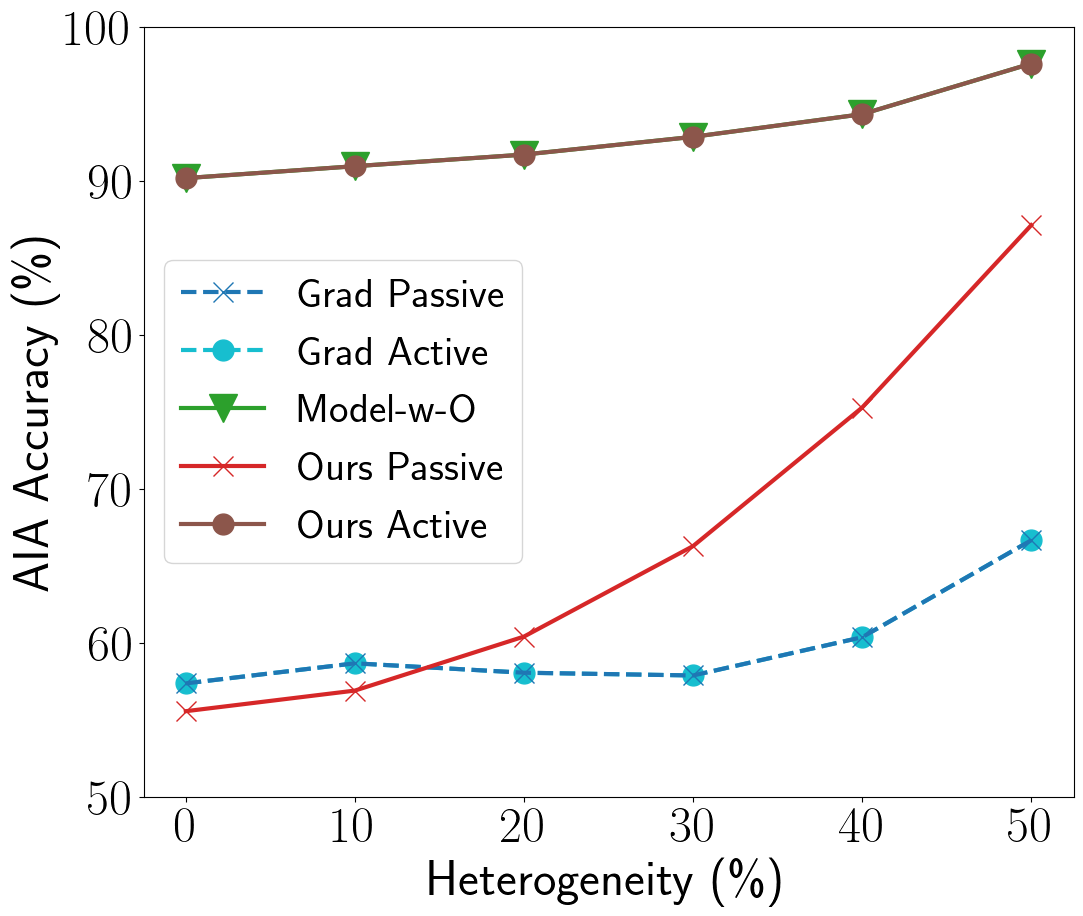
\includegraphics[scale=0.18]{assets/chapter_2/Heter_effect_louisiana_32.png}
\end{minipage}
\begin{minipage}[b]{0.33\linewidth}
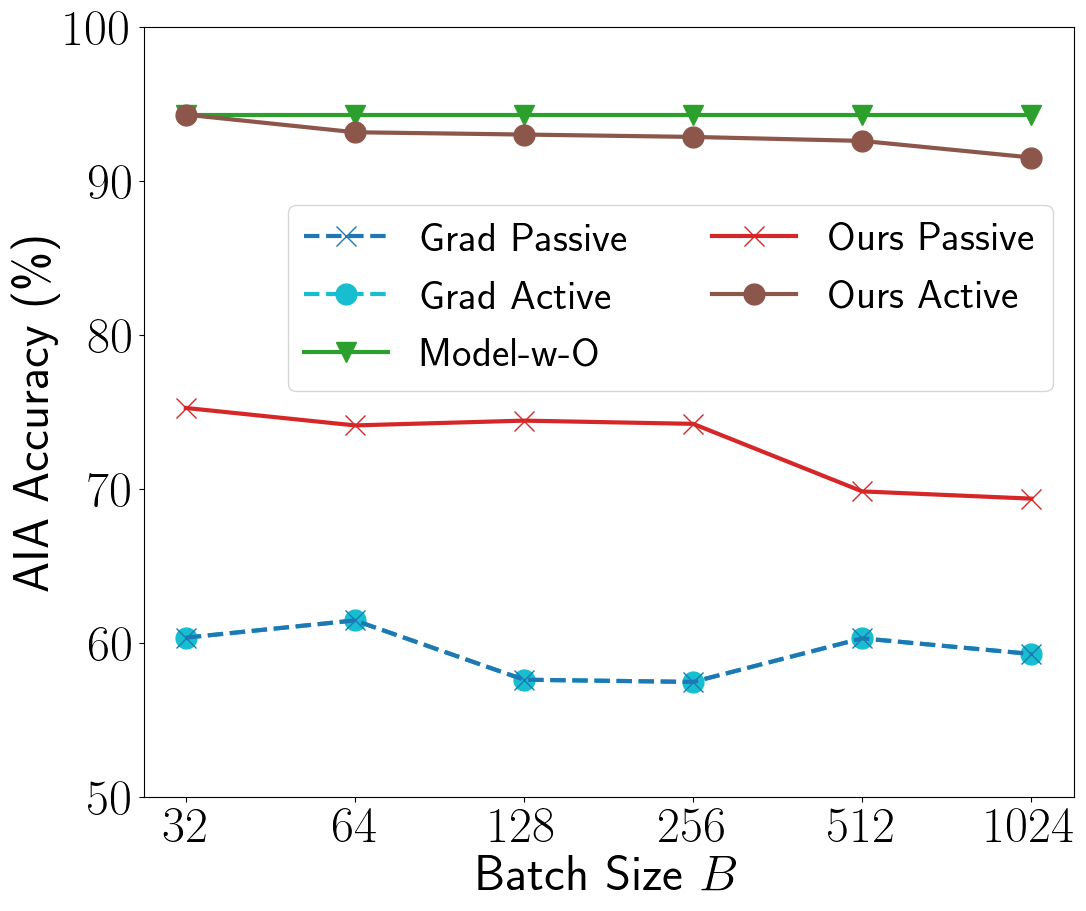
\includegraphics[scale=0.18]{assets/chapter_2/batch_size_effect_32.png}
\end{minipage}
\begin{minipage}[b]{0.33\linewidth}
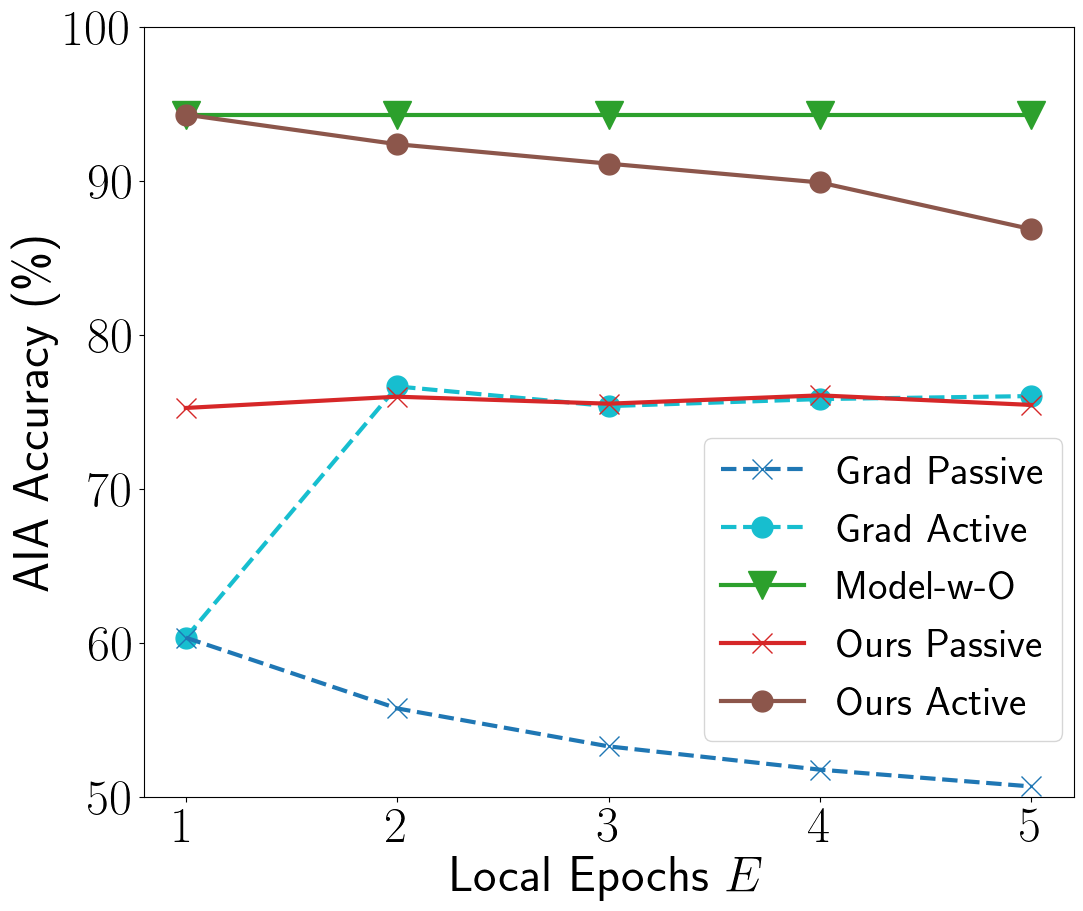
\includegraphics[scale=0.18]{assets/chapter_2/local_epochs_effect.png}
\end{minipage}
\caption{The AIA accuracy over all clients' local datasets under different heterogeneity levels (left) ($0\%$ represents i.i.d case), batch sizes (center), and local epochs (right) for Income-L dataset. The default values for heterogeneity level, batch size $B$ and local epochs $E$ are set to $40\%$, $32$, and $1$, respectively. The malicious adversary attacks $\lceil 50/E \rceil$ rounds after $\lceil 100/E \rceil $ communication rounds.
Crosses represent passive attacks, while dots represent active attacks. Dashed lines correspond to gradient-based attacks (Grad), and solid lines correspond to model-based attacks (Ours and Model-w-O).}
    \label{fig:impact}
\end{figure*}

\subsubsection{Impact of Data Heterogeneity} 
We simulate varying levels of heterogeneity in the Income-L dataset and illustrate how the attack performance evolves in Figure~\ref{fig:impact} (left). First, we observe that as the data is more heterogeneously split, the accuracy of AIA improves for all approaches. 
Indeed, the data splitting strategy (Appendix~\ref{app:datasplit_incomel}) leads to a greater degree of correlation between the clients' sensitive attributes and the target variable at higher levels of heterogeneity. This intrinsic correlation facilitates the operation of all AIAs.
We observe in these experiments, as in previous ones, that active Grad does not necessarily offer advantages over passive Grad. In the more homogeneous case (which is less realistic in an FL setting), our passive attack performs slightly worse than Grad, but its accuracy increases more rapidly with heterogeneity, resulting in an AIA accuracy advantage of over 20 p.p. in the most heterogeneous case.
Our active attack over 50 additional rounds consistently outperforms Grad by at least 30 p.p. and is almost indistinguishable from \mbox{Model-w-O}.

\subsubsection{Impact of Batch Size} 
%We test the FedAvg training with 1 local epoch and 6 different batch sizes. 
Figure~\ref{fig:impact} (center) shows that the performance of our attacks slightly decrease as the batch size increases.  A possible explanation for this is that a larger batch size results in fewer local updates per epoch, leading the client to return a less overfitted model. Despite this, our approach consistently outperforms Grad in all cases.
%This is due to the fact that a larger batch size results in fewer local updates per epoch, leading to the client returning a less over-fitting model. Despite this, our approach consistently outperforms Grad in all cases.
% NOTE: slightly reformulated to save enough space to fit in the number of pages.
\subsubsection{Impact of the Number of Local Epochs}
%We test the FedAvg training with batch size 32 and 5 different local epochs. 
Figure~\ref{fig:impact} (right) shows that under passive attacks our approach is not sensitive to the number of local epochs, whereas Grad's performance deteriorates to the level of random guessing as the number of local epochs increases to 5. Interestingly, active Grad significantly improves upon passive Grad as the number of local epochs increases. While our active approach progressively performs slightly worse, it still maintains an advantage of over 10 p.p.~compared to Grad.

\subsubsection{Impact of the Local Dataset Size}
Figure~\ref{fig:dataset_size_effect} shows how each client's dataset size impacts individual (active) AIA accuracy in Income-A dataset. %The experiment setting is the same as in Table~\ref{tab:attacks_32} with  50 active rounds.
We observe that for all methods, clients with smaller datasets are more vulnerable to the attacks,  
%Because the corresponding gradients incorporate less samples and 
because the models overfit the dataset more easily. 
Moreover, for clients with over 20000 data points, Grad provides an attack performance close to random guessing.
\begin{figure}[ht]
    \centering
    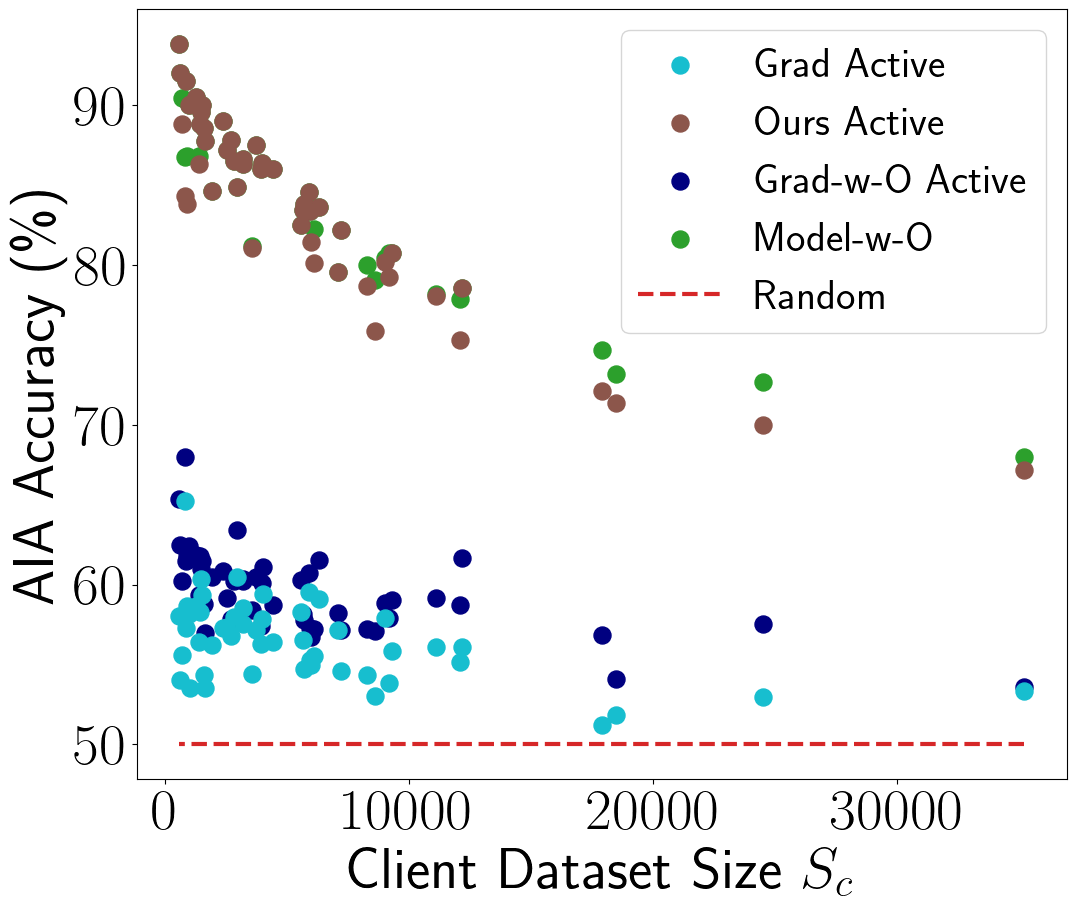
\includegraphics[scale=0.2]{assets/chapter_2/client_acc_scatterplot.png}
    \caption{AIA accuracy in Income-A dataset on clients with different local dataset size $S_c$. The experiment setting is the same as in Table~\ref{tab:attacks_32} with  50 active rounds.}
    \label{fig:dataset_size_effect}
\end{figure}

\subsubsection{Impact of Differential Privacy}
To mitigate privacy leakage, we apply a federated version of DP-SGD \cite{Abadi_dp}, providing sample-level differential privacy guarantees~\cite{Dwork, slDP}. 
Our experiments show that, even with this defense mechanism in place, our approach still outperforms the baselines in most of the scenarios.  Results are in Appendix~\ref{app:defense}.

\section{Discussion and Conclusions}
In our work, we have demonstrated the effectiveness of using model-based AIA for federated \emph{regression} tasks, when the attacker can approximate the optimal local model. For an honest-but-curious adversary, we proposed a computationally efficient approach to reconstruct the optimal \emph{linear} local model in least squares regression. In contrast, for neural network scenarios, our passive approach involves directly utilizing the last returned model (Sec.~\ref{subsec:baseline}). We believe more sophisticated reconstruction techniques may exist, and we plan to investigate this aspect in  future work.

The reader may wonder if the superiority of model-based attacks over gradient-based ones also holds for \emph{classification} tasks. Some preliminary experiments we conducted suggest that the relationship is inverted. We advance a partial explanation for this observation.
 For a linear model with binary cross-entropy loss, it can be shown that the model-based AIA \eqref{eq:aia_model_based} on a binary sensitive attribute is equivalent to a simple label-based attack, where the attribute is uniquely reconstructed based on the label. This approach leads to poor performance because the attack relies only on general population characteristics and ignores individual specificities.
This observation also holds experimentally for neural networks trained on the Income-L dataset, largely due to the inherent unfairness of the learned models. For example, for the same set of public features, being a man consistently results in a higher probability of being classified as wealthy compared to being a woman. As a consequence, the AIA infers gender solely based on the high or low income label. These preliminary remarks may prompt new interesting perspectives on the relationship between fairness and privacy (see for example the seminal paper~\cite{chang2021privacy}).

% NOTE: Modification here, removed description of mixup and tappfl
Finally, to mitigate privacy leakage, beyond differential privacy mechanisms, there are empirical defenses such as Mixup~\cite{mixup}, and TAPPFL~\cite{aaai_defense}. However, the effectiveness of these defenses has not yet been demonstrated on \emph{regression} tasks, and we leave this for future work.
